%!TEX TS-program = xelatex
%!TEX encoding = UTF-8 Unicode

%\def \papersize {a4paper}
\def \papersize {letterpaper}

\documentclass[12pt,\papersize]{extarticle}
% extarticle is like article but can handle 8pt, 9pt, 10pt, 11pt, 12pt, 14pt, 17pt, and 20pt text

\def \ititle {Motor representation in goal ascription}
\def \isubtitle {}
\def \iauthor {}
\def \iauthor {C. Sinigaglia* \& S. Butterfill**
\\ 
**Dipartimento di Filosofia, Università degli Studi di Milano, Italia
\\ 
***Department of Philosophy, University of Warwick, UK}
\def \iemail{corrado.sinigaglia@unimi.it}
%\date{}

\input{$HOME/Documents/submissions/preamble_steve_paper3}
%\author{}
%\author {S. Butterfill* \& C. Sinigaglia**
%\\ 
%**Department of Philosophy, University of Warwick, UK
%\\ 
%***Dipartimento di Filosofia, Università degli Studi di Milano, Italia}
%\date{}


\begin{document}

\setlength\footnotesep{1em}

\bibliographystyle{newapa} %apalike

\maketitle
%\tableofcontents
\title{}



% --- paste from google docs after here ---






\begin{abstract}
\noindent
%
How could judgements about the goals of actions depend on motor representations? Many findings show that they do, but several obstacles ... Overcome obstacles by showing that motor representations support experiences of action in something like the ways in which visual representations support experiences of objects ... Implications for mindreading.
%

\ % blank line

\noindent
Key words: ***

\ % blank line

\noindent
Word count: ***
\end{abstract}

\tolerance=5000








\section{Introduction}


Motor processes sometimes occur in action observation and facilitate judgements about the goals to which actions are directed (see section \vref{sec:evidence} and \citealp{rizzolatti_functional_2010} for a review). 
Suppose you observe someone's hand moving towards a pair of scissors. 
You may judge that she will shortly perform an action directed to cutting something up. 
Making this sort of judgement is sometimes facilitated by the occurrence of motor processes \citep{boria:2009_intention, ortigue:2010_understanding}.  
This is not to say that it would be altogether impossible to make a judgement of this type without the involvement of motor processes. 
What the evidence shows is rather that judgements about the goals of actions are sometimes faster or more accurate (or both) when motor processes occur in action observation than when they do not.
How could this work? 
How could motor processes sometimes facilitate judgements about the goals to which actions are directed?

Our aim in this paper is to answer this question. 
The first step is to ask about the contents of motor representations.
Where judgements about the goals of observed actions depend on the observers' motor representations, what do those motor representations represent?
To understand how goal ascription judgements could depend on motor representations we need to understand how the contents of the motor representations compare with the contents of the judgements.
In section \vref{sec:content} we aim to remedy this need by identifying evidence for two claims. First, some motor representations represent not merely kinematic or dynamic features of actions but outcomes to which actions are directed. Second, although the directedness of an action to an outcome cannot be represented motorically, it can be captured by motor processes which determine how an action should unfold in order for the outcome to be realised. So the status of a particular motor representation as a representation of a goal to which an action is directed depends both on its content---on its being a representation of an outcome---and on its role in motor processes which determine how that action should unfold.
We propose that where a judgement about the goal to which an action is directed depends on motor representations, there is a motor representation of an outcome which captures the directedness of the action to the goal.

The second step in our attempt to understand how some judgements depend on motor representations concerns the apparent isolation of motor representation from thought. When judgements about the goals of observed actions depend on the observers' motor representations, which processes connect motor representations to judgements?
We shall argue (in section \vref{sec:processes} that motor representations are related to experiences.  There is a parallel between visual and motor representations. Visual representations of the particular colours of objects are related to experiences of those objects and their colours, and these experiences arguably provide reasons for judgements about the colours of objects.%
\footnote{
*Some controversy.  Campbell: yes; Davidson: no (experience plays a merely causal role).  We simply assume yes.  (Or we can duck: we're talking about appearance to the thinker of having reasons, not the fact of having reasons.)}
So the fact that visual representations enable judgements about particular colours in no way conflicts with the claim that thinkers have reasons for those judgements.  We shall argue that motor representations of outcomes are related to experiences of actions and their directedness to outcomes.  This is why thinkers can have reasons for judgements about the directedness of an action to a goal even where the judgements are enabled by motor representations---and also why it appears (veridically) to thinkers that they have such reasons.  Motor representation stands to experience of action as visual representation stands to experience of particular colours. This anyway is the view we shall defend.

This view has implications for understanding how goal ascription relates to mindreading. A familiar view in philosophy has it that goal ascription depends on the ascription of intentions, which in turn is interdependent with ascriptions of belief and desire (*refs). On this view goal ascription is possible only as part of a larger mindreading project. By contrast we shall show that in some cases the only representations involved in goal ascription are motor representations. So goal ascription can occur independently of any knowledge of mental states. It is therefore coherent to conjecture that facts about the goals of actions form part of the evidential basis for mental state ascription. Knowledge of others' minds ultimately depends on knowledge of their actions, which in turn depends on experiences made possible by motor representations.  Mindreading starts from motor experiences of actions.

***NOTE: There is not enough about the importance of the question and its wider philosophical significance.

[*rephrase (also introduction): there is evidence that is naturally interpreted as showing that motor representation facilitates judgements about the goals to which actions are directed. But there is also an obstacle to accepting this conclusion: it is unclear how this could occur.  In this paper we aim to remove the obstacle by explaining how motor representation could facilitate judgements about the goals of actions.]


\section{Does motor representation sometimes facilitate action judgements?}
\label{sec:evidence}

Before launching into the main task for this paper we shall briefly review evidence for our opening premise. Why suppose that motor representation sometimes facilitates judgements about the goals to which actions are directed?

As a preliminary, note that it is now well established that motor processes and representations are involved not only in producing actions but also in observing actions. Indeed there seem to be some striking similarities between the sorts of processes and representations usually involved in performing a particular action and those which typically occur when observing someone else perform that action \citep{rizzolatti_functional_2010,rizzolatti_mirrors_2008}. 

If motor representations occur in action observation, then observing actions might sometimes facilitate performing compatible actions and interfere with performing incompatible actions.  Both effects do indeed occur, as several studies have shown \citep{brass:2000_compatibility, craighero:2002_hand, kilner:2003_interference, costantini:2012_does}. To give just one example, \citet{kilner:2003_interference} asked subjects to move their arms horizontally while they observed another person moving their arms either horizontally (that is, congruently) or vertically (that is, incongruently). They found that subjects' movements deviated significantly more when observing incongruent actions, and much as they would deviate if the subjects had been required to move their other arm incongruently. The effect cannot be explained as a consequence of observing mere movements because the same effect was not found when subjects observed a robot moving its arm.

Of course the fact that motor representation occurs in action observation does not show, further, that motor representation actually facilitates judgements about the goals to which actions are directed.  

What would count as evidence for this further claim that motor representation can facilitate goal ascription?  One possible source of evidence involves motor expertise. If manipulating subjects' motor expertise can selectively affect their abilities to identify the goals of actions, this would be evidence that motor representation sometimes facilitates goal ascription.  Accordingly, \citet{casile:2006_nonvisual} asked subjects to make judgements about observed actions, including were some that are typically difficult to perform without training.  These actions were presented to subjects as point-light stimuli to ensure that only visual information about the actors' joint displacements was available.%
\footnote{
Readers who unfamiliar with point-light stimuli may view examples at http://www.biomotionlab.ca/Demos/BMLwalker.html.
The technique was introduced by \citet{johansson:1973_visual}.
}
They compared performance before and after subjects were trained to perform those actions themselves. They found that subjects' ability to accurately judge which action was being performed improved with the training. This is plausibly a consequence of increased motor expertise rather than any form of perceptual learning because the subjects were blindfolded during training (and the point-light stimuli on which their judgements were based are, of course, entirely visual). A related way to measure the effects of motor representation on judgements is to temporarily lesion part of the motor cortex using repetitive transcranial magnetic stimulation  \citep{urgesi:2007_representation, moro:2008_neural}.  \citet{urgesi:2007_representation} measured how long subjects took to make judgements about the type of action they were observing. They found that a temporary lesion to the premotor cortex, but not a temporary lesion to another brain area, increased the time taken to make action judgements. And the effect of lesioning the premotor cortex was specific to action judgements: subjects' abilities to make observational judgements identifying body parts was unaffected. Putting these studies together, we have evidence that enhancing motor representation (through training) sometimes facilitates judgements about the goals of actions, while destroying motor representation even temporarily can impair such judgements.

Further evidence comes from  studies of neurological deficits. If deficits in abilities to perform certain actions specifically impair abilities to make observational judgements about actions of that type, this would also indicate that motor representation can facilitate action judgements.  \citet{serino:2009_lesions_} compared the performances of control and hemiplegic subjects who were asked to identify actions. They found that ability to perform an observed action was correlated with ability to recognise that action. In particular, hemiplegic subjects were less accurate in identifying actions performed with limbs on the hemiplegic side of their bodies than actions performed with limbs on the unaffected side. By contrast, no such pattern was found for control subjects, which included both a group of healthy subjects and also a group of brain-damaged patients with no motor deficit.  (Including the latter group makes it possible to rule out the possibility that the findings were due to a general deficit in higher-order visual processing). Other evidence for a role for motor representation in judgements of action comes from research on apraxia. In one study subjects were asked to identify actions such as cutting paper and drinking with a straw on the basis of the sounds these actions produced. Subjects with limb apraxia showed an impairment in recognising hand-related actions (such as cutting paper) whereas subjects with buccofacial apraxia were impaired in recognising mouth-related actions (such as drinking); but no subjects showed a general impairment in recognising sounds and their significance \citep{pazzaglia:2008_sound_}. These links between motor deficits and action judgements provide further evidence that motor representation sometimes facilitates action judgements.%
\footnote{
In addition to facilitating judgements about the goals of observed actions, motor representations and processes may also sometimes facilitate judgements about the possibility of performing an action \citep{grosjean:2007_fitts_law, eskenazi:2009_role}.
}

Motor representation may not always be necessary for observational judgements about the goals of actions. Indeed, as \citet{mahon:2008_action} notes, some studies suggest that apraxic subjects can recognise actions they cannot perform \citep[see also][]{hickok:2009_eight}. This is consistent with our premise that motor representation sometimes facilitates judgements about actions.  Even if this facilitation were an extremely rare phenomenon, the question of how it is possible would still arise.



\section{What can motor representations represent?}
\label{sec:content}

We have just reviewed evidence that judgements about the goals of actions  are sometimes facilitated by motor representation. Our project is to understand how this could happen.  A first step is to understand how the contents of the judgements compare with the contents of motor representations. Where judgements about the goals of actions depend on motor representations, could those motor representations represent outcomes to which the actions are directed?  In this section we argue for a positive answer on the grounds that some motor representations do represent outcomes and that there are processes which ensure that, in observing an action, the outcomes represented motorically are normally outcomes to which the observed action is directed. This will allow us to conclude that motor representations can facilitate judgements about goals in part because some motor representations represent outcomes which are among the goals of the actions.  

We take for granted that action observation sometimes involves motor representations of merely kinematic features of actions.  For example, when observing someone about to press a button, it may be useful to be able to identify with some degree of precision the trajectory her finger will follow and how long it will take to reach the button. In some cases observers represent both features of such actions motorically (*ref). But our concern is with the further claim that some motor representations represent outcomes. 

How can we distinguish a representation of an outcome from a representation of merely kinematic features of actions? This is possible because a single outcome can be realised by actions with quite different kinematic features and, conversely, actions with arbitrarily similar kinematic features can realise different outcomes in different contexts.  To illustrate, consider this outcome: the grasping of a particular pen. This could be realised by any of at least three types of action which vary kinematically: a hand action, a foot action or a tool-using action.  If we had marks we could use to identify motor representations independently of knowing their contents, and if we had evidence that these marks were constant across instances of all three types of action, then we could infer that some motor representations capture something more abstract than the kinematic features particular to the hand, foot or tool-using action. But we do have well established marks of motor representation, for motor representation can be inferred from patterns of neuronal discharge, from motor-evoked potentials, from where blood flows in motor areas of the brain, from behavioural performance profiles and in other ways besides.  And we do have evidence that such marks are constant across instances of all three types of action which realise the grasping outcome \citep{rizzolatti:1988_functional, Rizzolatti:2001ug, cattaneo:2010_state-dependent}. So we can infer that some motor representations do not represent merely kinematic features of actions. To infer, further, that some motor representations represent outcomes we need to consider what happens where, conversely, we hold kinematic features constant while varying to which outcome an action is directed. Take an action which realises the grasping of a particular pen and compare it with a second action which is as similar as possible to the first with respect to its kinematic features but differs with respect to which outcome it is directed to because the pen is manifestly absent (so the action is not plausibly directed to grasping anything) or because the pen is manifestly too large or too small to grasp.  Some marks of motor representations distinguish these actions \citep{Umilta:2001zr, villiger:2010_activity, koch:2010_resonance}.  This together with the constancy of some motor representations across variations in kinematic features is good (if not conclusive) evidence that some motor representations represent outcomes to which actions are directed.%
\footnote{
We offer only a brief argument for this conclusion here because \citet{pacherie:2008_action} and \citet{butterfill:2012_intention} also argue for it; the latter further support this conclusion by appeal to the functions of motor processes in planning and monitoring action.
}

So far we have been arguing that some motor representations are about outcomes by contrasting this claim with the hypothesis that all motor representations concern merely kinematic features of action.  This is not quite enough for a convincing argument because some people have argued, convincingly, that some motor representations in some way concern sensory consequences of actions (*refs).
To illustrate, grasping a small ball between your finger and thumb will have predictable tactile and visual consequences, and it is possible (at least in principle) that some motor representations involved in grasping the ball might somehow concern these sensory consequences.
Note that the outcomes to which actions are directed are often distinct from any of the action's sensory consequences.
Take grasping a ball again: although the outcome---the grasping of the ball---reliably has sensory consequences, these are neither necessary nor sufficient for the outcome to occur.  
They are not necessary because grasping could also be performed with a foot or a tool, which could substantially alter the sensory consequences of the action; and because grasping could also in principle occur in complete darkness with numb hands.%
\footnote{
Here we leave open the question of whether there are actions with certain  proprioceptive sensory consequences that are necessary for the action to occur. 
} 
The sensory consequences are also not sufficient because in principle the pattern of movements of finger and thumb in relation to the ball could occur without there being any event directed to the grasping of an object---such movements might in principle occur as part of an exercise in moving one's fingers in which the ball is an unwanted distraction rather than a target.
So our claim that motor representations represent outcomes is conceptually quite distinct from the claim that some motor representations might in some way concern sensory consequences of actions: in principle, both claims might be true, or one might be true while the other is false.

Suppose, at least for the sake of argument, that some motor representations do indeed somehow concern sensory consequences of actions. 
Do we still have grounds for holding that there are motor representations of outcomes?  Yes.  We noted just above that it is possible to vary the sensory consequences of an action while holding one of its outcomes constant.  
To return to the example, grasping a ball can be done with a hand, a foot or a tool.
Using different effectors will alter how the action looks (its visual consequences), sounds and feels but not the goal to which it is directed. 
So the fact that observing instances of all three types of action can involve a common motor representation shows that not all motor representations concern either sensory consequences or merely kinematic features only.  
Motor representations of outcomes are also needed.

The claim that some motor representations represent outcomes raises a further question.  Which outcomes can be represented motorically?  
This question arises because actions are typically directed to many outcomes.  For instance, a single action might be directed to grasping the scissors, to cutting a newspaper and to removing a particularly useful article to file later.  In reaching for the scissors the agent is already performing actions directed to all of these outcomes.  Which outcomes can be represented motorically?  Not all outcomes can be represented motorically, of course.  For instance, the difference between cutting out an article and cutting out a picture from a newspaper is not a difference that need be captured by any motor representations.  One idea about which outcomes can be represented motorically starts from the observation that outcomes can be partially ordered by the means-end relation. It might be assumed that motor representations capture only least outcomes relative to the means-end ordering.  This is wrong, however.  Differences such as that between reaching for a pair of scissors to cut something and reaching for a pair of scissors to place them somewhere (perhaps to put them away) are captured by motor representations (\citealp{Fogassi:2005nf, cattaneo:2007_impairment, bonini:2010_ventral}). This suggests that motor representations are not limited to representing least outcomes.  


\section{How to capture the directedness of a goal-directed action}
Our overall question is how motor representation could facilitate judgements about the goals of observed actions. We have just argued that motor representations which occur in action observation can represent outcomes. Now it would be natural to suppose that these outcomes are sometimes outcomes to which the observed actions are directed, and that this is no accident.  But the argument so far provides no clue as to what might ensure this, as it is silent on processes linking the outcome represented to the observed action.  What (if anything) ensures that an outcome represented motorically in action observation is an outcome to which the observed action is directed?  

To see the force of this question, note that there is a distinction between merely representing outcomes---which may in fact be outcomes to which certain actions are directed---and representing outcomes as outcomes to which a particular action is directed. This point applies to representations generally, including both motor representations and intentions.  For instance, you might know that a friend intends to break an egg (and so represents an outcome, namely an egg's breaking) and see the friend handling an egg which breaks without yet knowing whether this breaking was appropriately related to that intention.  To represent an outcome and an action does not necessarily involve representing any relation between them.  Our first task, then, is to consider whether some motor representations might somehow represent, not merely outcomes, but also the directedness of particular actions to certain outcomes.  

But how might the directedness of an action to an outcome be represented? The notion of goal-directedness is standardly explained in terms of intention: for an action to be directed to an outcome is for the action to be appropriately related to an intention whose content specifies that outcome (or, on some views, an intention specifying an appropriately related outcome---see \citealp{Bratman:1984jr}). Given this view, no motor representation could represent the directedness of an action to an outcome.  After all, no motor representation represents an intention.  

There are, of course, other attempts to explicate the notion of goal-directedness.  For instance, some have argued that the directedness of some actions to particular outcomes can be explained in terms of motor representation and not only in terms of intention \citep{butterfill:2012_intention}.  This changes nothing, however.  For motor representations do not represent any representations at all.  So the directedness of an action to an outcome cannot be represented motorically.

One way to avoid our argument for this conclusion would be to claim that the directedness of an action to a goal can be understood in ways that do not involve intention or any representation at all.  For instance, consider the idea that an action's being directed to an outcome may consist in its having the function of bringing about that outcome, where function might be construed teleologically.%
\footnote{
Teleological accounts of function, and of the application of this notion to understanding goal-directed action, have been extensively developed (*see further Godfrey-Smith 1996; Millikan 1984; Neander 1991; Price 2001; Wright 1976).
} 
Even if we accepted this idea, we would still have to conclude that motor representations do not represent goal-directedness. After all, motor representations no more represent functions than they represent representations.

If, as we have suggested, motor representations can represent outcomes but not the directness of actions to outcomes, what (if anything) might ensure that, when someone observes a particular action, outcomes she represents motorically are outcomes to which that action is directed? We must face this question because if it turned out that it was only ever a coincidence that outcomes represented motorically in action observation are outcomes to which the observed action is directed, then it would be hard to understand the role of motor representation in facilitating judgments. In the rest of this section we shall argue that the directedness of an action to an outcome could be captured motorically by means of a planning-like process which involves determining how an outcome is to be achieved and whether given movements are appropriate to achieving that outcome.

To see how this might work, let us step back, momentarily, from motor phenomena to introduce the idea with an illustration.  Observing Ayesha gathering some papers during a long meeting that shows no sign of ending, you conjecture that a goal of these and her next actions will be to leave discretely. You use this conjecture about the outcome to which Ayesha's actions are directed to determine one or more likely sequences of behaviours, almost as if you were planning from her point of view how to achieve that outcome. This leaves you with expectations concerning how she will act. You might be waiting for Ayesha, who has no other friends present, to give you a nod before quietly pushing away from the table. If what you observe matches these expectations, or if there are only deviations that can be explained in ways consistent with your conjecture about the goal of Ayesha's actions, then you may come to regard the conjecture as confirmed. But if there is a mismatch---if, for example, Ayesha signals that she wants attention and looks around to check people are looking at her---then you might reject the conjecture about the goal of her actions being to leave discretely. As this illustrates, determining how an action will or would unfold and then monitoring how it does unfold can ensure that there is a reliable connection between the action's being directed to a certain outcome and your representing that outcome. So the directedness of an action to a goal can be captured by a planning-like process together with appropriate monitoring.

In outline the link between an action and an outcome to which it is directed can be maintained like this. The representation of an outcome leads to a planning-like process which generates predictions about how the action will unfold, and this representation is weakened to the extent that the predictions are not met.  This is how planning processes can be coopted to ensure that an outcome represented is likely to be an outcome to which the observed action is directed.

Could motor processes capture the directedness of an action to an outcome in this way? In action observation it is not just that there may be motor representations of outcomes. There is also evidence that a motor representation of an outcome sometimes causes a determination of which movements are likely to be performed to achieve that outcome  \citep{kilner:2004_motor, urgesi:2010_simulating}. The processes involved in determining how observed actions are likely to unfold given their outcomes are closely related, or identical, to processes involved in performing actions. This is suggested both by the involvement of regions of the brain associated with action (*refs), and by patterns of facilitation and interference which occur when simultaneously observing and performing actions \citep{brass:2000_compatibility, kilner:2003_interference, craighero:2002_hand}. It is almost as if the observer were planning the agent's actions. 

Planning-like processes in action observation have also been demonstrated by measuring observers’ predictive gaze.  If you were to observe just the early phases of a grasping movement your eyes may jump to its likely target, ignoring nearby objects \citep{ambrosini:2011_grasping}. These proactive eye movements resemble those you would typically make if you were acting yourself \citep{Flanagan:2003lm}: in reaching for something, it is natural to look at the target rather than your hand.  Importantly, the occurrence of such proactive eye movements in action observation depends both on representing the outcome of an action (even temporary interference in the observer's ability to represent the outcome will interfere with the eye movements, \citealp{Costantini:2012fk}) and also on planning-like processes (requiring the observer to perform actions incongruent with those she is observing also interferes with proactive eye movements, \citealp{Costantini:2012uq}).  This, then, is further evidence that observers do something almost like planning the actions they observe.  

We can now see how motor processes might ensure that an outcome represented is likely to be an outcome to which the observed action is directed.  As we have seen, there is evidence that observers represent outcomes motorically and that planning-like processes generate expectations about how the actions will unfold given these outcomes.  To take a tiny step further, we conjecture that, in action observation, motor representations of outcomes are weakened to the extent that the expectations they generate are unmet \citep[compare][]{Fogassi:2005nf}. This is how the directedness of action to an outcome can be captured motorically even in the absence of any representation of intention or function.

Let us sum up so far. Our overall question is how motor representations could ever facilitate judgements about the goals of actions.  Our focus until now has been relations between the contents of judgements and the contents of motor representations.  
In the previous section we argued that the contents of some motor representations cannot be fully characterised in terms of merely kinematic features and sensory consequences of action only; rather, some motor representations represent outcomes to which actions are directed.  
This led us to ask, in the present section, what if anything ensures that outcomes represented motorically in action observation are outcomes to which the observed action is directed.  We argued that motor representations probably do not represent the directedness of an action to an outcome, but explained how directedness can be captured by planning-like motor processes which occur in action observation.  Potentially, then, there is a respect in which the content of a motor representation may resemble the content of judgement about the goal to which an action is directed: there may be an outcome which both represent, and both may  capture the directedness of an action to that outcome.  
We therefore conjecture that where motor representation facilitates a judgement about the goal to which an action is directed, there is a motor representation of this outcome, or of a related outcome, and a planning-like process which captures the directedness of the action to the outcome.  Motor representations can facilitate judgements about the goals of actions because the goals can be represented motorically and because the directedness of actions to those goals can be captured motorically.

This conjecture, however, far from fully answering our overall question, throws up a further challenge.  For the conjecture, that motor representation facilitates judgements partly by virtue of the contents of motor representations matching those of judgements, implies that there are content-respecting influences of motor representation on judgement.  The existence of such content-respecting influences is surprising given that motor representations are to a significant degree isolated from judgements. True, the evidence all but forces us to accept that such influences occur.  But that leaves us with the question of how such influences are possible. How could motor representations sometimes have content-respecting influences on judgements?  What might connect some privileged motor representations to judgements about goals in action observation?%
\footnote{
At this point it may be tempting to make a radical move by supposing that there are direct inferential relations between motor representation and thought.  But the evidence we have reviewed does not support this radical move, and there are compelling arguments for denying that motor representations are inferentially integrated with the thoughts involved in explicit judgements about the goals of observed actions (see e.g.\ \citealp{butterfill:2012_intention}).
 Note also that someone who made this radical move would have to explain why motor representation and judgement appear to be inferentially isolated in many other cases.}


\section{***Notes for Action Experience section}


DUSSELDORF ARGUMENT (rough, from Friday skype):
(1) Motor imagery involves experience of action as such (e.g. of grasping as such) and not just of sensory consequences of actions
(one relevant consideration is that you know not only which action you are imagining but when you have succeeded in imagining performing it);
(corollary: there can be experiences of action without experiences of acting)
(2) There are common elements between what you  experience when you imagine acting and what sometimes you experience when you observe an action; in particular, the experience of action is common to both
Therefore
(3) Sometimes observing action involves experiencing action as such



------- there is evidence that motor representation might have content-respecting influences on judgment

MR ----?----- JUD
  experience: how to argue 
….............how is possibile? experience revelatory of action
------------------- parallel between colour and action experience

TBE: content-respecting influences of (MR of G$_1$) onto (Jud about G$_2$) where G$_1$ matches G$_2$


Explanation-1: MR of G captures directedness of action a -> experiences of action a as directed to G -> judgement that action is directed to goal G
	Key component: Dusseldorf argument, imagination

Explanation-2: MR of G captures directedness of action a -> experiences revelatory of action but experiences as of sensory consequences of actions -> association between experienced sensory consequences and action directed to goal G (how? for example, I know the sound of a newspaper being opened) -> judgement that action a is directed to goal G

E.g. clapping:
	representation of sound
	representation of action
	association: characteristic sounds<>action
	Thanks to the association, experience of the sounds can result in a representation of the action



\section{***NEW PLAN***}
\begin{enumerate}
\item There is experience revelatory of action
	\begin{enumerate}
	\item there is a phenomenal element which is common to : (i) performing, (ii) imagining and (iii) observing action
	\item this common phenomenal element enables us to know (i) which action we are performing, (ii) which action we are imagining, and (iii) which action we are observing.  It is an experience revelatory of action.
	\item the common phenomenal element depends on motor representation of an outcome to which the action is directed.  (This what links the motor representation to the experience).
	\end{enumerate}

\item What is this experience revelatory of action, and how does it explain the existence of content-respecting influences of motor representation on judgements about the goals of actions?
	\begin{enumerate}
	\item Indirect hypothesis: the experience revelatory of action is an experience of the movements involve in acting, or of sensory consequence of action

	\item Direct hypothesis: the experience revelatory of action is an experience of goal-directed action as such
	\end{enumerate}


\end{enumerate}


\section{Experience of Action}
\label{sec:processes}
Our aim in this and the following sections is to explore how motor representations could sometimes have content-respecting influences on judgements about the goals of observed actions. Broadly, our proposal is that the influence of motor representation on observational judgements goes via experience.  It is because motor representations can affect our experiences when we observe actions that those motor representations can facilitate judgements about the actions. 

Our argument will involve three steps. The first step is to argue that in performing, imagining and observing actions alike there are \emph{experiences revelatory of action}, that is, experiences which provide the subject of experience with reasons for correct judgements about which action someone is performing.  (Note that we initially leave open the question of what experiences revelatory of action are experiences of.)  The second step is to show that these experiences depend on motor representations.  And the third step is to consider what experiences revelatory of action could be experiences of, which is necessary in order to describe how all of this can be used to explain the existence of content-respecting influences of motor representation on judgements about the goals of actions.

When acting it is often possible to know which action you are performing---to know, for example, whether you are grasping a particular mug or stroking the cat (or perhaps both). How could you know this?  In some cases it might depend on knowing your intentions. However, there are cases in which people act on an intention but do something not compatible with fulfilling the intention (*ref). Suppose you are facing a mug and holding a wine glass for a friend and intend to grasp the mug but, perhaps due to being distracted or a manipulation of your attention, start to drink from the wine glass.  In such a case it is possible that you will realise what you are doing, stop it and attempt once more to grasp the mug. So you know what you are doing even though, in this sort of case, such knowledge does not plausibly depend on knowing what you intend.  A natural thought, then, is that in performing an action such as grasping, it is sometimes possible to know what you are doing on the basis of experience. That is to say, in acting there are (at least sometimes) experiences revelatory of action. This much should be almost uncontroversial.

Against this conclusion, someone may insist that knowledge of what you are doing depends on knowledge of your intentions even when distracted.  On this view, someone who intends to do one thing but absent mindedly starts to drink from a wine glass she is holding for a friend really intends to drink and knows that she intends this. But now consider the special case of a subject with anarchic hand syndrome who attempts to picks up a cup of tea with one hand while using the other hand to put the tea back onto the table.%
\footnote{
\citet[p.\ 1114]{della_sala:1991_anarchic}. Subjects with anarchic hand syndrome, which usually follows lesions of the anterior part of the corpus callosum and of the supplementary motor area, perform actions incompatible with their avowed intentions. These patients may also refer the their anarchic hand as having a mind of its own. he anarchic hand syndrome \citep{della_sala:1994fk}.
} 
%
This subject knows which actions she is performing with which hands: this knowledge is guiding her actions insofar as she uses one hand to control the other.  But it seems unlikely that this knowledge depends on knowing what she intends.  For she does not intend one of the actions she is performing, as she herself claims.  Or else, contrary to her own reports, she knowingly has an irrational combination of intentions; but such combinations of intentions do reliably generate detailed predictions about actions and so knowledge of these intentions could not explain the subject's knowledge of her own actions.  Either way, then, experience is needed to explain the possibility of knowing which actions one is performing.  This strengthens the conclusion that, at least sometimes, performing actions involves experiences revelatory of actions.  








\section{Experience of Action [*OLD]}
\label{sec:processes}
Our aim in this and the following sections is to explore how motor representations could sometimes have content-respecting influences on judgements about the goals of observed actions. Broadly, our proposal is that the influence of motor representation on observational judgements goes via experience.  It is because motor representations can affect our experiences when we observe actions that those motor representations can facilitate judgements about the actions. However this broad idea is consistent with two quite different hypotheses concerning the experiences associated with motor representation in action observation. 

One hypothesis, call it the Indirect Hypothesis, is based on evidence that, in observing action, motor representation can influence visual and acoustic experiences (see figure \vref{fig_indirect_hypothesis}). (Perhaps this holds for other modalities too.) The relevant experiences are perceptual experiences of bodily configurations and movements as an action unfolds, and perceptual experiences of characteristic sensory effects of actions.  Such experiences sometimes enable an observer to make judgements about the goals of actions, for she may associate particular patterns of bodily movement or particular sensory effects with particular goals.  But in many cases of action observation, the agent's bodily movements and the sensory effects of her actions may be partially obscured or surrounded by irrelevant distractors, or otherwise difficult to identify.  But suppose that, as some evidence suggests, motor representation can influence---and even enhance---such experiences of bodily configurations and movements, and of sensory effects.  Then motor representations might thereby facilitate judgements about the goals of actions.  So on the Indirect Hypothesis, motor representations sometimes enhance perceptual experiences of movements or sensory effects which in turn sometimes facilitate judgements about the goals of actions.   

\begin{figure}
\begin{center}
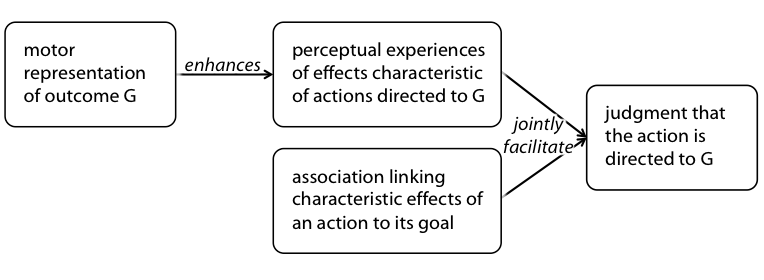
\includegraphics[width=\textwidth]{fig_indirect_hypothesis.png}
\caption{
\label{fig_indirect_hypothesis}
	The Indirect Hypothesis.
}
\end{center}
\end{figure}


To illustrate, suppose that an observer can associate the characteristic sound of a newspaper being snapped open with the action of snapping open a newspaper. Suppose also that, when observing an action, motor  representations can influence whether, when or how this observer experiences this characteristic sound.  Then motor processes can indirectly influence the speed and accuracy of the observer's judgements about which actions are directed to this goal, the snapping open of a newspaper, by influencing whether, when or how she experiences the characteristic sound of this action.%
\footnote{
The Indirect Hypothesis is inspired by and consistent with views defended in \citet{Csibra:2007fy} and \citet{Wilson:2005qu}.  However, to our knowledge these authors have not considered exactly our question about content-respecting influences of motor representation on judgement, and we are not suggesting that the would endorse the Indirect Hypothesis in its entirety.  
}


The other hypothesis is in some ways more radical.  This hypothesis, call it the Direct Hypothesis, is that in observing action we experience not only movements and sounds but also goal-directed actions as such (see figure \vref{fig_direct_hypothesis}). Such experiences---call them motor experiences---stand to motor representations somewhat as visual experiences stand to visual representations.  The motor experience of an action as directed to a particular outcome is made possible by a motor representation of that outcome.  So motor representations can have a content-respecting influence on judgements because motor representations enable motor experiences on which the judgements can be  based.  Or so the Direct Hypothesis claims.%
\footnote{
In formulating the Direct Hypothesis we draw on ideas from \citet{rizzolatti_mirrors_2008} and \citet{Jeannerod:1999kj}.
}

\begin{figure}
\begin{center}
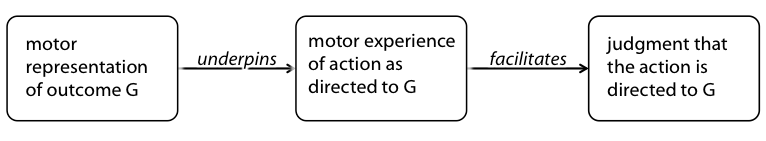
\includegraphics[width=\textwidth]{fig_direct_hypothesis.png}
\caption{
\label{fig_direct_hypothesis}
	The Direct Hypothesis.
}
\end{center}
\end{figure}


Let us say that an experience, motor or not, is \emph{revelatory of action} just if it can provide the subject of experience with reasons for correct judgements about which action someone is performing. On both hypotheses motor representations enable experiences which are revelatory of action. And both hypotheses use this broad idea to explain how motor representations could have content-respecting influences on judgements. The primary difference between the hypotheses concerns what these revelatory experiences are experiences of: whether all are experiences of movements, sounds and the like only (the Indirect Hypothesis), or whether some are experiences of goal-directed actions as such (the Direct Hypothesis).  

In the next section we expand on and consider evidence for the Indirect Hypothesis before turning to the Direct Hypothesis in the following section.



\section{The Indirect Hypothesis}
The Indirect Hypothesis depends on the claim that motor representations can influence perceptual experiences.  If this is right, we would expect to find that motor representation can have a content-respecting influence on perceptual processing. There is indeed evidence of such influences. For instance, \citet{bortoletto:2011_action} show that motor plans, such as might be involved in producing a gesture with the hand, can influence visual processes. Here the influence of motor representations on visual processes varies depending on both the gesture being planned and the visual stimulus presented. Importantly, these influences can be detected before any action occurs, showing that it is the motor representations rather than any consequent movements which are influencing visual processes.% 
\footnote{
For a recent review of some of the evidence concerning motor influences on perceptual processing, see \citet{halasz:2012_unconscious}. (*refs)
}  
This evidence shows that the claim about motor representations influencing experience is at least consistent with how motor and perceptual processes interact.

Of course, this evidence does not show that motor representation influences perceptual experiences.  After all, it may be possible to influence sensory processes in ways that make no difference to experience.  But there is also evidence that motor representation can influence perceptual judgements.  For some very special pairs of tones, the first is sometimes perceived as lower in pitch than the second and sometimes as higher in pitch.  Call these \emph{ambiguous tone pairs}.  Repp and Knoblich (\citeyear{repp:2007_action}) had a group of expert pianists and a control group of non-experts press two keys in sequence, where the first key was sometimes to the left, and sometimes to the right, of the second key.  The key presses produced an ambiguous tone pair, and the tones always occurred in the same order regardless of which key was pressed first.  By asking subjects to report how they perceived the relative pitch of the tones, Repp and Knoblich found that, for the expert pianists, the direction of the key presses influenced the perceived direction of the change in pitch. Could what influences perceptual experience in this case be not a motor representation but the occurrence of a movement, or perhaps even the perception of a movement of the subject's own fingers? Against this possibility, note that the effect was not observed in non-expert pianists: for them the direction of action did not measurably influence the perceived pitch direction. Since both groups moved in the same way, if the influence were due to movement only we would expect it to occur irrespective of expertise. Instead it seems likely that differences in expertise between the two groups of subjects, expert and non-expert, affected how the movements they performed were represented motorically, and that these differences in motor representation are in turn what explains their perception of relative pitch.  This study, and others like it,%
\footnote{
See also \citet{zwickel:2010_interference} who investigate effects of action on visual experience of motion.  *more \citep{schutz-bosbach:2007_perceptual}
} 
provide relatively direct evidence that motor representations can influence acoustic experiences.

How do these findings bear on the Indirect Hypothesis above, according to which motor representation in action observation enables experiences of sounds and movements that somehow facilitate the identification of actions?  Consider observing someone playing two notes on a piano.  Given that you know something about which sounds are produced by various piano playing actions, hearing the relative pitch of these notes might in principle assist you in recognizing that a goal of her action is to play these two notes.  So if, as the findings indicate, motor representation can influence perceptions of pitch, it might thereby indirectly facilitate judgements about the goals of actions.  

Of course the evidence we have considered leaves open the question of how extensive the influence of motor representations on perceptual experiences is.  For all we have said, such influences may be rare.  This is a potential problem for the Indirect Hypothesis, which requires such influences to occur in every case in which motor representation facilitates goal ascription.  However our aim in this paper is not to establish the correctness of an explanation but, more modestly, only to understand how motor representation could in principle facilitate judgements about the goals of actions.  Wilson and Knoblich (\citeyear{Wilson:2005qu}, p.\ 463) consider the possibility that motor representation may influence the representation of agents' bodies and their movements. They suggest that motor representation in action observation may help `to fill in missing or ambiguous information' and to project the likely course of an agent's bodily movements. This idea allows us to see that the Indirect Hypothesis is at least in principle capable of explaining how motor representation might facilitate goal ascription in a wide range of cases. Perhaps, then, motor representations of outcomes to which actions are directed influence---and even enhance---perceptual experiences of the agents' bodies and movements in ways that facilitate judgements about the goals of the actions.  So the Indirect Hypothesis.


MR--->PE of configuration \& movements ---->> Judg
MR ---> PE of pitch -->Judg about goal
Pitch: MR influence Perc [no action observation]



\section{The Direct Hypothesis: Experiences of Action}
Our aim is to understand how motor representations of outcomes can have a content-respecting influence on judgements about the goals of actions. 
According to the Direct Hypothesis, a motor representation of an outcome can underpin an experience of an action as directed to a matching outcome, and this experience can in turn ground a judgement about the goal of the action.  This hypothesis hinges on two potentially controversial claims.  The first is that in observing action we experience not only movements, sounds and other sensory effects of actions but also the goal-directed actions as such. And the second is that such experiences are underpinned by motor representations of corresponding outcomes.  

Is the first claim plausible?  Compare actually grasping a mug with merely imagining grasping it.  There is a way of imagining grasping the mug which resembles actually grasping it with respect to timing \citep{decety:1989_timing, decety:1996_imagined, Jeannerod:1994oz} and the sorts of factors that make acting more or less awkward \citep{parsons:1994_temporal, frak:2001_orientation}. Further, imagining grasping the mug in advance would bring some of the benefits of actually rehearsing grasping it (*ref). The experience involved in imagining grasping the mug in this way has something in common with the experience involved in actually grasping it.  But what is common to the two experiences?  

****

Is the first claim plausible?  First note that there is a phenomenologically action-like way of imagining, one which involves something almost like acting except that such imaginings are not necessarily responsive to the features of actual objects and do not necessarily result in bodily movements.  Suppose that you are about to perform a delicate operation with some scissors. You stand poised to act, but first pause to mentally pantomime performing the action. In some respects the experiences involved in this imaginative exercise may be barely distinguishable from experiences that might be involved in actually performing the operation (\citealp[p.\ 161]{currie:1997_mental}; \citealp[p.\ 727]{jeannerod:1995_mental}; \citealp[p.\ 638-9]{kosslyn:2001_neural}).  In fact, imagining performing the operation in advance has some of the benefits of actually rehearsing it (*ref).  For imagining performing an action in this phenomenologically action-like way sometimes resembles actually performing the action with respect to timing \citep{decety:1989_timing, decety:1996_imagined, Jeannerod:1994oz} and the sorts of factors that make acting more or less awkward \citep{parsons:1994_temporal, frak:2001_orientation}.  



Given that an experience of actually performing an action can have elements in common with the experience involved in merely imagining performing that action, what could these common elements be ?

Consider the following argument:
%
\begin{enumerate}
\item
In actually performing a goal-directed action it is sometimes possible experience the action as a goal-directed action.

\item
There is a way of imagining acting which involves something almost like acting, except that such imaginings are not necessarily responsive to the features of actual objects and do not necessarily result in bodily movements.

Therefore: sometimes, when you imagine performing an action you may experience a goal-directed action as such.

\item
What you experience when you imagine performing an action has elements in common with what you experience when you observe someone else performing that action; in particular, the experience of goal-directed action is common to both.
\end{enumerate}
Therefore:
\begin{enumerate}[resume]
\item
Sometimes observing a goal-directed action involves experiencing it as such.
\end{enumerate}
%
Without attempting to show that the premises are true, we shall offer some considerations which indicate that they are at least defensible. 

On the first premise, (1), we first need to distinguish two ways of imagining acting.  One, cognitive way of imagining involves something like thinking about performing an action.  Another, phenomenologically action-like way of imagining involves something almost like acting except that such imaginings are not necessarily responsive to the features of actual objects and do not necessarily result in bodily movements.  Suppose that you are about to perform a delicate operation with some scissors. You stand poised to act, but first pause to mentally pantomime performing the action. In some respects the experiences involved in this imaginative exercise may be barely distinguishable from experiences that might be involved in actually performing the operation (\citealp[p.\ 161]{currie:1997_mental}; \citealp[p.\ 727]{jeannerod:1995_mental}; \citealp[p.\ 638-9]{kosslyn:2001_neural}).  In fact, imagining performing the operation in advance has some of the benefits of actually rehearsing it.  For imagining performing an action in this phenomenologically action-like way sometimes resembles actually performing the action with respect to timing \citep{decety:1989_timing, decety:1996_imagined, Jeannerod:1994oz} and the sorts of factors that make acting more or less awkward \citep{parsons:1994_temporal, frak:2001_orientation}.  The first premise, (1), concerns this phenomenologically action-like way of imagining.  

Step 1: phenomenologically action-like imagination involves motor representation.  We know this because how actions unfold in this way of imagining reflects motor constraints linked to the goal of the action (so not only constraints arising from, for example, finger configuration) and timings.  For instance ...

Step 2: What do we experience when we imagine acting?  ***HERE
a.  There are no movements or sensory effects to experience (but there is  no action produced either).
b.  There is motor representation of action (but there may also be visual representation of sensory effects of the action not performed).
c.  I could be mistaken about the movements involved in an action and about its sensory effects but still know that I am imagining it (and not just because I intend to imagine it and then do some imaginative thing or other---if my mind wanders so that I start imagining a different action, I could know this).
(one relevant consideration is that you know not only which action you are imagining but when you have succeeded in imagining performing it); ()
(corollary: there can be experiences of action without experiences of acting)




We shall argue that acting sometimes involves experiences which can ground judgements about what one has done even though these are not experiences of movements or sounds.  In effect, the idea will be that you can strip away perceptual experiences and still be left with experiences revelatory of action.  These can only be experiences of action, or so we claim.  Two phenomena are involved in making this argument.  The first is anosognosia for hemiplegia, which shows that there can be experiences revelatory of action even in the absence of any actual movements.  The second is deafference, which confirms that these experiences are unlikely to be illusory experiences of movement. Together these phenomena support the view that, in performing actions, we have experiences of actions and not only of movements, sounds and the like.  

The argument sketched so far concerns experiences associated with performing actions, not observing them.  Note, however, that the basis of these experiences of action is motor representation and planning.  Since these are the very things which, in action observation, underlie the experiences enabling one to identify actions, it is reasonable to conclude that there is a phenomenal element common to performing an action and observing an action performed, namely the action itself.  Roughly, what you experience in performing an action is what you would experience if you were observing it.  But this is all to come; let us start by introducing some background. 

Anosognosia for hemiplegia is a clinical condition in which patients deny, and appear largely unaware of, a severe paralysis of one or more limbs on one side of their body.  It typically follows a stroke involving damage to motor areas in the right hemisphere of the brain (*refs).  To illustrate the effects of this condition, consider a subject with anosognosia for hemiplegia who was asked to brush her hair holding a brush in her contralesional hand.  Although she was unable to move the hand, she proceeded to move her head as if her hair were being brushed, and then reported having successfully brushed her hair \citep{berti:2008_motor}. This form of anosognosia cannot be explained as entirely due to neglect or complete ignorance of part of one's body \citep[p.\ 165]{berti:2008_motor}.  

Could anosognosia for hemiplegia be explained as mere confabulation or a top-down effect of judgement on experience?  This is incompatible with the performance of anosognosics on bimanual tasks \citep{berti:2008_motor, garbarini:2012_moving}.  To illustrate, consider an anosognosic who has been asked to wash with both hands.  Although she can only actually move one hand, she may move this hand in much the way that she would do if she were actually washing with both hands (*ref: personal communication?).  This is hard for ordinary subjects to reproduce (try it). For a more carefully controlled illustration, consider anosognosic subjects who were asked to draw simultaneously with both hands, one hand was supposed to continuously draw a vertical line and the other hand to continuously draws a circle.  Anosognosic subjects can of course only actually move one hand, but they show interference as if both hands were actually being moved.  That is, if you were to perform this task, your vertical line would become somewhat oval; this interference is an effect of bimanual coordination.  The striking finding is that anosognosic subjects show the same pattern of interference although not actually drawing a circle.  By contrast, subjects with motor neglect and subjects with hemiplegia but no anosognosia do not show this pattern of interference \citep{garbarini:2012_moving}.  This suggests that anosognosia involves relatively detailed action-related experiences and cannot be entirely explained as confabulation.  

On the leading, best supported explanation, anosognosia for hemiplegia arises from defects in monitoring action.  When a subject with anosognosia for hemiplegia is asked to perform an action involving a hemiparetic limb, motor planning occurs as it might do in ordinary subjects. Now in ordinary subjects, and in hemiplegic subjects without anosognosia, the predicted effects of a planned action are compared with motor representations of action outcomes.  Consequently if such subjects tried and failed to initiate an action, they would normally be aware of their failure even without seeing or touching their limbs. However, in anosognosic subjects the comparator is damaged and no signal of failure is generated.  This is why it seems to them that they have acted despite failing even to initiate the action.  Of course, anosognosic subjects can perceive that their objectives have not been met: after apparently opening a bottle, for instance, they can see that the bottle remains shut; they would not normally proceed to drink from it.  And these subjects do not necessarily have visual, proprioceptive or tactile sensory impairments.  But the experience associated with motor planning dominates, so that it seems to them as if they have acted.  From their point of view, it seems that the bottle is peculiarly difficult to open rather than that they are unable to move a limb \citep[pp.\ 173-4]{berti:2008_motor}.  

How is anosognosia for hemiplegia relevant to the issue of whether there are experiences of action as such?  It seems that anosognosic subjects have some experiences which are revelatory of action---revelatory in the sense that they provide reasons for judgements about actions---despite not actually moving a limb.  What could these experiences be experiences of?  Consider the claim that these are experiences of movement only.  While it is arguably not generally correct to infer an absence of experience of movement from the absence of actual movement, in this particular case it does seems unlikely that there could be experience of movement.  After all, some anosognosic subjects have intact perceptual systems: if they experience movement at all, they should experience an absence of movement.  So any experiences of movement will not be the sort of experiences that would provide reasons for judgements about successful action.  Given that (as argued above) the experiences on which anosognosic subjects' judgements of action are based are also not entirely a product of confabulation, it is plausible to accept that they are experiences of action as such.

This view is further supported by research on deafferented subjects.  These subjects lack tactile and proprioceptive sensory feedback from their actions but, unlike subjects with anosognosia for hemiplegia, can actually move their limbs.  Such subjects may continue to have some experiences characteristic of action; for instance, when asked to flex an index finger they can report having done so even in the absence of visual information \citep{kristeva:2006}.  These subjects' sensory deficits make it unlikely that their experiences could be of movements or the like (*no: motor-perception associations; but what do they report?): it is more plausible that, concerning acting, their experiences are like those of subjects with anosognosia for hemiplegia.  None experience movement: what they experience is action.

Anosognosia and deafference comprise a useful pair of cases: some anosognosics we have preserved perceptual senses and an absence of actual bodily movement, whereas individuals suffering deafference have damaged senses and actual bodily movement.  But in both cases there are experiences revelatory of action.  The existence of these disorders indicates that motor representation is sufficient for experiences capable of grounding judgements about actions even in the absence of any perceptual experiences of movements, sounds or the like.  It is plausible to infer that these experiences are experiences of action as such.

***HERE: todo.  Two things.  First, explain the timing experiment---it's not all about subjects with brain damage, there is converging evidence from ordinary subjects.  Second, explain the comparitor model.  

***Anosognosia for hemiplegia : experience of action without acting (cannot be an experience of movement, \&c).  Or could this be an illusory experience of one's body moving?  \citep{garbarini:2012_moving}%
\footnote{
See also \citet{gallese:2010_bodily}: "Brugger, Kollias, Muri, Crelier, and Hepp-Reymond (2000) described one of these cases. fMRI imaging of their patient during phantom limb sensations of hand movements showed activation of premotor and posterior parietal cortex. Aplasic phantoms can therefore be explained as the phenomenal correlate of planning/monitoring action of an absent limb."}
and hand-washing: \citep{berti:2008_motor}

***parallel with speech (short)



\section{Conclusion}
Motor representation enables judgements about the goals of actions by making possible experiences of action as such.  

\subsection{Reasons}
In making judgements about the goals of actions, it appears (perhaps veridically) to the thinker that she has reasons for those judgements, much as it appears to her that she has when making visual judgements about the particular colours of objects.  Or, if we are sceptical about thinkers having reasons for visual judgements, at least we can say that it does not seem to the thinker that she is simply landed with the judgement.  Contrast someone who `knew at a glance' that a vase is genuine Ding ware, or someone on a blind date who, on first catching sight of her partner for the night, `just knows' that this is the one she wants to spend the rest of her life with.  Action judgements often seem different from these: rather than simply being landed with them, it may seem to a thinker that they bear a straightforward relation to her experience. 

Our view is consistent with the claim that it appears to a thinker that she has reasons for making judgements about the goals of actions even when  those judgements depend on motor representations.
  Motor representation stands to experience of action as visual representation stands to experience of particular colours. 


\subsection{Goal ascription without metarepresentation}
Having noted above that goal ascription often or always involves representing the directedness of an action to an outcome, we argued that this is something no motor representation can represent. Equally, however, we noted that the directedness of actions to outcomes can be captured by planning-like processes, and we suggested that motor representations can feature in such processes.  One possibility, then, is that there might be a kind of goal ascription---or something resembling goal ascription---where the only representations involved are motor representations.  This enables us to see how there could be goal ascription, or something very like it (we are not insisting that the term 'goal ascription' be used) could occur without metarepresentation. This gives us a first role for motor representation in goal ascription which distinguishes motor representation from representations of intentions or other mental states.  Where goal ascription involves capturing the directedness of actions to goals by representations of intentions it thereby involves metarepresentation; but where the only representations involved in goal ascription are motor representations, there is no metarepresentation at all.











\section{* PLAN *}
[Corrado's Challenge: Why is this not just about implementation details?]
\begin{enumerate}
\item What roles, if any, might motor representation play in goal ascription?
\item Some motor representations occur in action observation and sometimes facilitate goal ascription (Serino; basketball; \& others?) (otherwise the question would be bizarre).  This is what makes the question pressing (timely).
\item The Question: How is this possible?  How could motor representation facilitate goal ascription?
\item Philosophical motivation: A familiar view in philosophy has it that goal ascription depends on the ascription of intentions, which in turn is interdependent with ascriptions of belief and desire (*refs). On this view goal ascription is possible only as part of a larger mindreading project. By contrast, developmental psychologists have assumed that goal ascription is possible even without knowing anything of an agent's mental states (*refs).  Our concern is with this pure form of goal ascription, goal ascription that occurs independently of knowledge of mental states.
\item There are two problems.  (a) adequacy of motor representation; (b) link between motor representation and judgement about the action and its goal
\item Problem (a).  Motor representations may represent outcomes but not the directedness of actions to outcomes?
\item Solution to problem (a): Capturing vs. representing the directedness of actions.
\item Problem (b): If we thought of motor representation as cut off from experience, it would seem impossible that differences in motor representation could make a difference to the reasons available from the observer's point of view.  
\item However, there is evidence that motor representation influences experience (e.g. acoustic experience of pitch direction).
\item One possibility: motor representation influences visual and acoustic experiences of movements and sounds, and these somehow facilitate goal ascription
\item This does not seem to be a fully adequate explanation because ?
\item Furthermore, motor representation enables experience which are (i) revelatory of action and (ii) distinct from visual or auditory experiences (Berti \&c).
\item So maybe: motor representation enables experiences of action as such
\item Conclusion: motor representation enables goal ascription by making possible experiences of action as such.  The role of motor representation in goal ascription is like the role of visual representation in judgements of motion.
\end{enumerate}

MR----> | acquisition| Action Judgment (action concept) <----> B \& D Judgment (b\&d concept)
tracking goal -----> || ascribing goal <----------------- > ascribing beliefs and desires

MR<----> Action Judgment (action concept) <----> B \& D Judgment (b\&d concept)






\bibliography{$HOME/endnote/phd_biblio}



\end{document}


